
\section{Experiments}\label{section:exp}

In this section, we compare our proposed DeepFM and the other state-of-the-art models empirically. The evaluation result indicates that our proposed DeepFM is more effective than any other state-of-the-art model and the efficiency of DeepFM is comparable to the best ones among the others.

\subsection{Experiment Setup}\label{sec:exp:set}

\subsubsection{Datasets}\label{sec:exp:set:data}

We evaluate the effectiveness and efficiency of our proposed DeepFM on the following two datasets.

\noindent\textbf{1) Criteo Dataset}: Criteo dataset \footnote{http://labs.criteo.com/downloads/2014-kaggle-display-advertising-challenge-dataset/} includes 45 million users' click records. There are 13 continuous features and 26 categorical ones. We split the dataset randomly into two parts: 90\% is for training, while the rest 10\% is for testing.

\noindent\textbf{2) Company$\ast$ Dataset}: In order to verify the performance of DeepFM in real industrial CTR prediction, we conduct experiment on Company$\ast$ dataset. We collect 7 consecutive days of users' click records from the game center of the Company$\ast$ App Store for training, and the next 1 day for testing. There are around 1 billion records in the whole collected dataset. In this dataset, there are app features (e.g., identification, category, and etc), user features (e.g., user's downloaded apps, and etc), and context features (e.g., operation time, and etc).

\subsubsection{Evaluation Metrics}\label{sec:exp:set:metric}

We use two evaluation metrics in our experiments: \textbf{AUC} (Area Under ROC) and \textbf{Logloss} (cross entropy).

\subsubsection{Model Comparison}\label{sec:exp:set:comparemodel}

We compare 9 models in our experiments: \textbf{LR}, \textbf{FM}, \textbf{FNN}, \textbf{PNN (three variants)}, \textbf{Wide \& Deep}, and \textbf{DeepFM}. In the Wide \& Deep model, for the purpose of eliminating feature engineering effort, we also adapt the original Wide \& Deep model by replacing LR by FM as the wide part. In order to distinguish these two variants of Wide \& Deep, we name them LR \& DNN and FM \& DNN, respectively.\footnote{We do not use the Wide \& Deep API released by Google, as the efficiency of that implementation is very low. We implement Wide \& Deep by ourselves by simplifying it with shared optimizer for both deep and wide part.}

\subsubsection{Parameter Settings}\label{sec:exp:set:hyper}

To evaluate the models on Criteo dataset, we follow the parameter settings in \cite{pnn} for FNN and PNN: (1) dropout: 0.5; (2) network structure: 400-400-400; (3) optimizer: Adam; (4) activation function: tanh for IPNN, relu for other deep models. To be fair, our proposed DeepFM uses the same setting. The optimizers of LR and FM are FTRL and Adam respectively, and the latent dimension of FM is 10.

To achieve the best performance for each individual model on Company$\ast$ dataset, we conducted carefully parameter study, which is discussed in Section~\ref{sec:exp:hyper}.
%We present in Table~\ref{table:comhyper} the hyper-parameters of deep models that can achieve the best performance on Company$\ast$ dataset.
%
%\begin{table}[ht]
%
%\centering
%%\scriptsize
%\caption{Hyper-parameters of deep model on Company$\ast$}\label{table:comhyper}
%\begin{tabular}{|c|c|c|c|}
%\hline
%
%&Activate&&Model \\
%&Function&Dropout&Structure \\ \hline
%FNN  & relu & 0.8 & 150-300-150\\ \hline
%IPNN  & tanh & 0.9 & 400-400-400\\ \hline
%OPNN   & relu & 0.6 & 500-400-300\\ \hline
%PNN$\ast$  & relu & 0.8 & 100-200-300\\ \hline
%LR \& DNN   & relu & 0.7 & 400-400-400\\ \hline
%FM \& DNN   & relu & 0.8 & 900-800-700\\ \hline
%DeepFM  & relu & 0.9 & 400-400-400\\ \hline
%\end{tabular}
%\end{table}

\subsection{Performance Evaluation}\label{sec:exp:perfor}

In this section, we evaluate the models listed in Section~\ref{sec:exp:set:comparemodel} on the two datasets to compare their effectiveness and efficiency.

\subsubsection{Efficiency Comparison}\label{sec:exp:perfor:time}

The efficiency of deep learning models is important to real-world applications. We compare the efficiency of different models on Criteo dataset by the following formula: $\frac{|training\ time\ of\ deep\ CTR\ model|}{|training\ time\ of\ LR|}$. The results are shown in Figure~\ref{fig:time}, including the tests on CPU (left) and GPU (right), where we have the following observations:
1) pre-training of FNN makes it less efficient;
2) Although the speed up of IPNN and PNN$\ast$ on GPU is higher than the other models, they are still computationally expensive because of the inefficient inner product operations;
3) The DeepFM achieves almost the most efficient in both tests.

%Test on CPU suggests that efficiency rank of the models is: LR \& DNN, OPNN, DeepFM, FM \& DNN, FNN, PNN$\ast$, IPNN. This rank is consistent with our theoretical analysis: pre-training of FNN makes it less efficient; IPNN and PNN$\ast$ are computationally expensive because of the inefficient inner product; OPNN is much faster than the IPNN and PNN$\ast$ because of computation approximation. Although DeepFM is only ranked the third place over all the 7 deep models, the difference between DeepFM and the winner LR \& DNN is minor.
%
%GPU is able to accelerate the matrix multiplication of inner product significantly, therefore the speed up of IPNN and PNN$\ast$ is higher than the other models. Even so, the efficiency order of the models is changed slightly: OPNN, DeepFM, FM \& DNN, LR \& DNN, PNN$\ast$, FNN, IPNN. As we can see, in GPU environment, the pre-training of FNN makes it even more unacceptable to use in real cases. The DeepFM achieves almost the best performance in terms of efficiency.

\begin{figure}[ht]
\setlength{\abovecaptionskip}{0pt}%
\setlength{\belowcaptionskip}{-10pt}
\centering
\begin{minipage}[b]{0.5\textwidth}
\includegraphics[width=0.45\textwidth]{img/cpu-time.png}
\includegraphics[width=0.45\textwidth]{img/gpu-time.png}
\end{minipage}
\caption{\footnotesize{Time comparison.}}\label{fig:time}
\end{figure}

\subsubsection{Effectiveness Comparison}
The performance for CTR prediction of different models on Criteo dataset and Company$\ast$ dataset is shown in Table~\ref{table:performance}, where we have the following observations:
\begin{itemize}
\item Learning feature interactions improves the performance of CTR prediction model. This observation is from the fact that LR (which is the only model that does not consider feature interactions) performs worse than the other models. As the best model, DeepFM outperforms LR by 0.86\% and 4.18\% in terms of AUC (1.15\% and 5.60\% in terms of Logloss) on Company$\ast$ and Criteo datasets.
\item Learning high- and low-order feature interactions simultaneously and properly improves the performance of CTR prediction model. DeepFM outperforms the models that learn only low-order feature interactions (namely, FM) or high-order feature interactions (namely, FNN, IPNN, OPNN, PNN$\ast$). Compared to the second best model, DeepFM achieves more than 0.37\% and 0.25\% in terms of AUC (0.42\% and 0.29\% in terms of Logloss) on Company$\ast$ and Criteo datasets.
\item Learning high- and low-order feature interactions simultaneously while sharing the same feature embedding for high- and low-order feature interactions learning improves the performance of CTR prediction model. DeepFM outperforms the models that learn high- and low-order feature interactions using separate feature embeddings (namely, LR \& DNN and FM \& DNN). Compared to these two models, DeepFM achieves more than 0.48\% and 0.33\% in terms of AUC (0.61\% and 0.66\% in terms of Logloss) on Company$\ast$ and Criteo datasets.
\end{itemize}
%Table~\ref{table:performance} presents the overall performance of different models on Criteo dataset and Company$\ast$ dataset. As can be observed, DeepFM outperforms all the other models in terms of AUC and Logloss, on both datasets. This improvement empirically verifies our theoretic analysis when we design DeepFM in Section~\ref{section:App}. DeepFM achieves better performance than LR, FM, FNN and PNN, due to the fact that DeepFM considers both high- and low-order feature interactions when making prediction. Moreover, DeepFM outperforms LR\&DNN and FM\&DNN, because DeepFM shares the feature embedding between deep and FM component which makes the feature representation more precise.

\begin{table}[ht]
\centering
\footnotesize
\caption{\footnotesize{Performance on CTR prediction.}}\label{table:performance}
\begin{tabular}{|c|c|c|c|c|}
\hline
\multirow{2}{*}{} & \multicolumn{2}{c|}{Company$\ast$} & \multicolumn{2}{c|}{Criteo} \\
 \cline{2-5}
 & AUC & LogLoss & AUC & LogLoss\\ \hline
LR      & 0.8640    & 0.02648   & 0.7686 & 0.47762\\ \hline
FM      & 0.8678    & 0.02633   & 0.7892 & 0.46077\\ \hline
FNN     & 0.8683    & 0.02629   & 0.7963 & 0.45738\\ \hline
IPNN    & 0.8664    & 0.02637   & 0.7972 & 0.45323\\ \hline
OPNN    & 0.8658    & 0.02641   & 0.7982 & 0.45256\\ \hline
PNN$\ast$    & 0.8672    & 0.02636   & 0.7987 & 0.45214\\ \hline
LR \& DNN & 0.8673    & 0.02634   & 0.7981 & 0.46772\\ \hline
FM \& DNN & 0.8661    & 0.02640   & 0.7850 & 0.45382\\ \hline
DeepFM  & \textbf{0.8715}    &  \textbf{0.02618}  & \textbf{0.8007} & \textbf{0.45083}\\ \hline
\end{tabular}
\end{table}


%the performance of FM is better than LR. Specifically, it is 0.58\% lower in terms of LogLoss and 0.43\% higher in terms of AUC than LR on Company$\ast$, and 3.53\% lower in terms of LogLoss and 2.68\% higher in terms of AUC than LR on Criteo. This improvement comes from the ability of FM to capture order-2 feature interactions automatically. In addition, when considering both low- and high-order feature interactions, DeepFM obtains the highest performance. It is 1.15\% lower in terms of LogLoss and 0.86\% higher in terms of AUC than LR on Company$\ast$, and 5.60\% lower in terms of LogLoss and 4.18\% higher in terms of AUC than LR on Criteo.


Overall, our proposed DeepFM model beats the competitors by more than 0.37\% and 0.42\% in terms of AUC and Logloss on Company$\ast$ dataset, respectively. In fact, a small improvement in offline AUC evaluation is likely to lead to a significant increase in online CTR. As reported in ~\cite{wide-n-deep}, compared with LR, Wide \& Deep improves AUC by 0.275\% (offline) and the improvement of online CTR is 3.9\%. The daily turnover of Company$\ast$'s App Store is millions of dollars, therefore even several percents lift in CTR brings extra millions of dollars each year.

\subsection{Hyper-Parameter Study}\label{sec:exp:hyper}

We study the impact of different hyper-parameters of different deep models, on Company$\ast$ dataset. The order is: 1) activation functions; 2) dropout rate; 3) number of neurons per layer; 4) number of hidden layers; 5) network shape.

\subsubsection{Activation Function}\label{sec:exp:hyper:act}

According to \cite{pnn}, \emph{relu} and \emph{tanh} are more suitable for deep models than \emph{sigmoid}. In this paper, we compare the performance of deep models when applying \emph{relu} and \emph{tanh}. As shown in Figure~\ref{fig:act}, relu is more appropriate than tanh for all the deep models, except for IPNN. Possible reason is that relu induces sparsity.

\begin{figure}[ht]
\setlength{\abovecaptionskip}{0pt}%
\setlength{\belowcaptionskip}{-10pt}
\centering
\begin{minipage}[b]{0.5\textwidth}
\includegraphics[width=0.48\textwidth]{img/act-auc.png}
\includegraphics[width=0.48\textwidth]{img/act-logloss.png}
\end{minipage}
\caption{\footnotesize{AUC and Logloss comparison of activation functions.}}\label{fig:act}
\end{figure}

\subsubsection{Dropout}\label{sec:exp:hyper:drop}

Dropout~\cite{dropout14} refers to the probability that a neuron is kept in the network. Dropout is a regularization technique to compromise the precision and the complexity of the neural network. We set the dropout to be 1.0, 0.9, 0.8, 0.7, 0.6, 0.5. As shown in Figure~\ref{fig:drop}, all the models are able to reach their own best performance when the dropout is properly set (from 0.6 to 0.9). The result shows that adding reasonable randomness to model can strengthen model's robustness.

\begin{figure}[ht]
\setlength{\abovecaptionskip}{0pt}%
\setlength{\belowcaptionskip}{-10pt}
\centering
\begin{minipage}[b]{0.5\textwidth}
\includegraphics[width=0.48\textwidth]{img/drop-auc.png}
\includegraphics[width=0.48\textwidth]{img/drop-logloss.png}
\end{minipage}
\caption{\footnotesize{AUC and Logloss comparison of dropout.}}\label{fig:drop}
\end{figure}

\subsubsection{Number of Neurons per Layer}\label{sec:exp:hyper:neuron}

When other factors remain the same, increasing the number of neurons per layer introduces complexity. As we can observe from Figure~\ref{fig:neuron}, increasing the number of neurons does not always bring benefit. For instance, DeepFM performs stably when the number of neurons per layer is increased from 400 to 800; even worse, OPNN performs worse when we increase the number of neurons from 400 to 800. This is because an over-complicated model is easy to overfit. In our dataset, 200 or 400 neurons per layer is a good choice.

\begin{figure}[ht]
\setlength{\abovecaptionskip}{0pt}%
\setlength{\belowcaptionskip}{-10pt}
\centering
\begin{minipage}[b]{0.5\textwidth}
\includegraphics[width=0.48\textwidth]{img/neuron-auc.png}
\includegraphics[width=0.48\textwidth]{img/neuron-logloss.png}
\end{minipage}
\caption{\footnotesize{AUC and Logloss comparison of number of neurons.}}\label{fig:neuron}
\end{figure}

\subsubsection{Number of Hidden Layers}\label{sec:exp:hyper:layer}

As presented in Figure~\ref{fig:layer}, increasing number of hidden layers improves the performance of the models at the beginning, however, their performance is degraded if the number of hidden layers keeps increasing. This phenomenon is also because of overfitting.

\begin{figure}[ht]
\setlength{\abovecaptionskip}{0pt}%
\setlength{\belowcaptionskip}{-10pt}
\centering
\begin{minipage}[b]{0.5\textwidth}
\includegraphics[width=0.48\textwidth]{img/layer-auc.png}
\includegraphics[width=0.48\textwidth]{img/layer-logloss.png}
\end{minipage}
\caption{\footnotesize{AUC and Logloss comparison of number of layers.}}\label{fig:layer}
\end{figure}

\subsubsection{Network Shape}\label{sec:exp:hyper:shape}

We test four different network shapes: constant, increasing, decreasing, and diamond. When we change the network shape, we fix the number of hidden layers and the total number of neurons. For instance, when the number of hidden layers is 3 and the total number of neurons is 600, then four different shapes are: constant (200-200-200), increasing (100-200-300), decreasing (300-200-100), and diamond (150-300-150). As we can see from Figure~\ref{fig:shape}, the ``constant" network shape is empirically better than the other three options, which is consistent with previous studies~\cite{networkstructure09}.

\begin{figure}[ht]
\setlength{\abovecaptionskip}{0pt}%
\setlength{\belowcaptionskip}{-10pt}
\centering
\begin{minipage}[b]{0.5\textwidth}
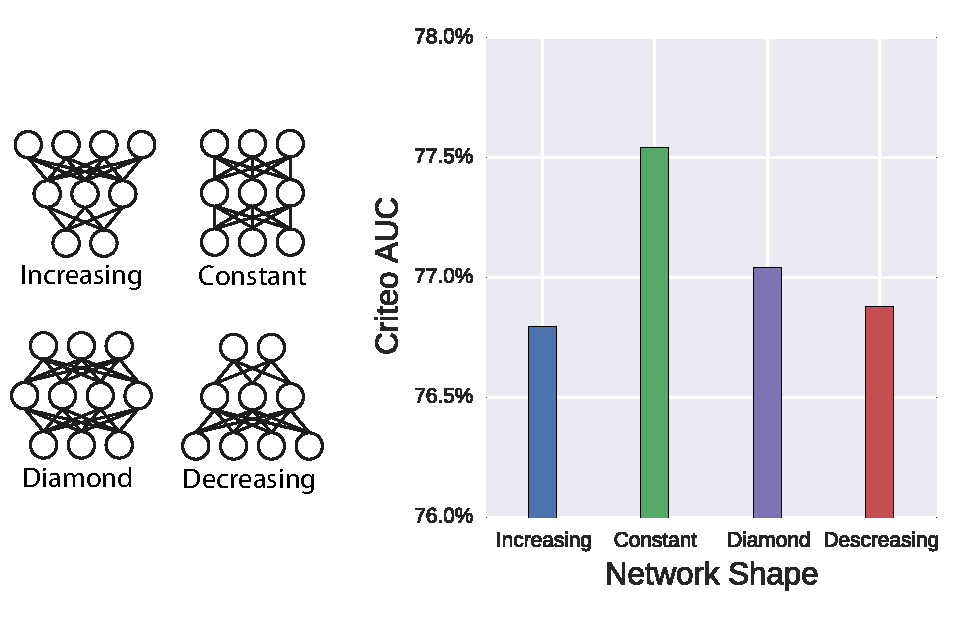
\includegraphics[width=0.48\textwidth]{img/shape-auc.png}
\includegraphics[width=0.48\textwidth]{img/shape-logloss.png}
\end{minipage}
\caption{\footnotesize{AUC and Logloss comparison of network shape.}}\label{fig:shape}
\end{figure}
